\documentclass[12pt,a4paper]{article}

\usepackage{color}
\usepackage{amsxtra}  
\usepackage{amsthm}
\usepackage{amssymb}
\usepackage{amsfonts}
\usepackage{graphicx}  
\usepackage{rotating}


\begin{document}

\title{Rouse theory of pinned polymer loop}
\author{Wenwen Huang}
\date{\today}

\maketitle

\section{Model}
\label{sec:model}

Consider a pinned polymer loop modeled by beads and connecting springs, see in
the sketch Fig. \ref{fig:beadSpring}.
\begin{figure}[htpb]
    \centering
    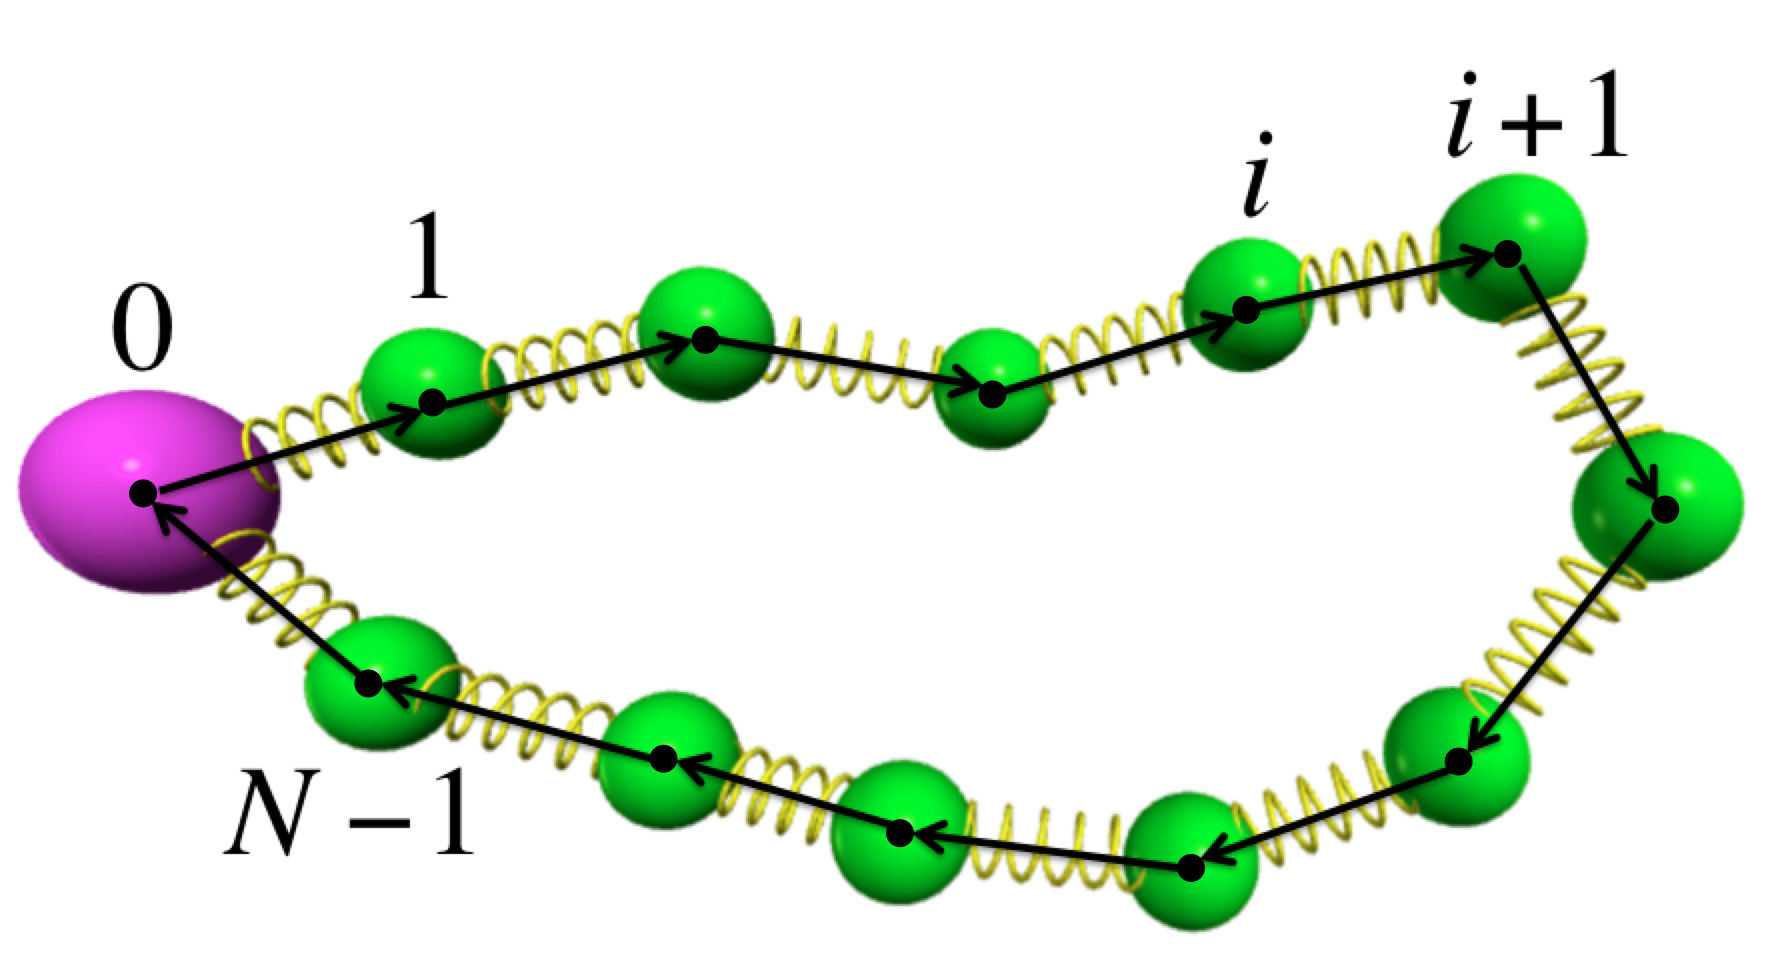
\includegraphics[width=0.8\linewidth]{beadSpring}
    \caption{Sketch of pinned bead spring model, magenta bead represent the
        pinned SPB, green beads represent chromosome segments.}
    \label{fig:beadSpring}
\end{figure}
Without loss of generality, the bead labeled by $0$ is assumed be pinned at the
origin and there are $N$ beads in total in the loop. We can write the pinned
condition as 
\begin{equation}
    \label{eq:pinCondition}
    \mathbf{r}_0 = \mathbf{0}
\end{equation}

So the dynamical equation for a single bead except the pinned one in the loop
can be written as 
\begin{equation}
    \label{eq:bead}
    \xi \frac{d \mathbf{r}_i}{dt} = - k_H \sum_{k} A_{ik} \mathbf{r}_k + \mathbf{f}_i^e + \mathbf{f}_i^b
\end{equation}
where $\xi$ is the friction coefficient of bead in solution, $\mathbf{r}_i$ is
the bead position of the $i$th bead, $k_H$ is the spring constant with a linear
Hookean spring assumed. $\mathbf{f}_i^e$ is the external force exerted on beads,
$\mathbf{f}_i^b$ is typical brownian force satisfying 
\begin{equation}
    \label{eq:brownian}
    \left<\mathbf{f}_i^b\right> = \mathbf 0; 
    \left<f_{i\alpha}^b(t)f_{j\beta}^b(t^\prime)\right> = 2\xi k_B T \delta_{ij}
    \delta_{\alpha\beta}\delta(t-t^\prime)
\end{equation}
$\mathbf A$ is the connecting matrix. It is not difficult to find that in the
case of the setting above, i.e. pinned loop, $\mathbf{A}$ is a $(N-1)\times
(N-1)$ matrix and has the following form
\begin{equation}
    \label{eq:connectMatrix}
    \mathbf{A} = \begin{bmatrix}
        2 & -1 & 0   & \cdots   \\
        -1 & 2 & -1  &  \cdots  \\
        \vdots & \ddots &\ddots&\vdots\\
        \cdots & -1 &2 & -1 \\
        \cdots & 0 &-1 &2
    \end{bmatrix}
\end{equation}

Notice that we do not take into account any complex terms of interaction such as
bending stiffness and exclusive effect in this simple model.  This is because
analytical results are tractable in such a simple setting. The impact of these
complex interaction terms will be studied numerically by Brownian Dynamics
Simulation.  

\section{Solution}
\label{sec:solution}

For convenience, we use the vector notation and rewrite Eq. \eqref{eq:bead} as 
\begin{equation}
    \label{eq:beadVector}
    \xi \frac{d }{dt} \mathbf{R} = - k_H \mathbf{A} \mathbf{R} + \mathbf{F}^e + \mathbf{F}^b
\end{equation}
where $\mathbf{R} = \left[\mathbf r_1, \mathbf r_2, \cdots, \mathbf r_{N-1}\right]^T$,
and similar vector notation is also applied for $\mathbf{F}^e$, $\mathbf{F}^b$.
In order to solve this set of dynamical equations, we first notice that the
connecting matrix $\mathbf{A}$ is a very special type of matrix called
tridiagonal Toeplitz matrix\cite{}. Luckily, it is always exactly
diagonalizable. To do this, let us introduce a similarity transfer that
\begin{equation}
    \label{eq:similarityTransfer}
    \left[\mathbf{\Omega}^{-1} \mathbf{A} \mathbf{\Omega}\right]_{jk} =
    \mathbf{D}_{jk} = \lambda_k\delta_{jk}
\end{equation}
here $\mathbf{\Omega}$ is normalized to be a unitary matrix, and $\lambda_k$ is the
eigenvalue of matrix $\mathbf A$. We skip the calculation details here and just give
out the results as following
\begin{eqnarray}
    \lambda_k  & = & 4\sin^2\left(\frac{k\pi}{2 N}\right), k = 1, 2, \cdots, N-1 \\
    \Omega_{jk} & = & \Omega_{kj} = [\Omega^{-1}]_{jk} = [\Omega^{-1}]_{kj} =
    \sqrt{\frac{2}{N}}\sin\left(\frac{jk\pi}{N}\right)
\end{eqnarray}
With this we can multiply both sides of Eq. \eqref{eq:beadVector} by
$\mathbf{\Omega}^{-1}$ arrive at
\begin{equation}
    \label{eq:badVectorTransfer}
    \xi\frac{d(\mathbf{\Omega}^{-1}\mathbf{R})}{dt} = -k_{H}\mathbf{\Omega}^{-1}
    \mathbf{A}\mathbf{\Omega}\mathbf{\Omega}^{-1}\mathbf{R} +
    \mathbf{\Omega}^{-1}\mathbf{F}^e + \mathbf{\Omega}^{-1}\mathbf{F}^b
\end{equation}
Notice that $\mathbf{\Omega}^{-1}\mathbf{A}\mathbf{\Omega} = \mathbf{D}$ and
use the notation such that $\tilde{\mathbf{R}} = \mathbf{\Omega}^{-1}
\mathbf{R}$, we get the set of decoupled equations
\begin{equation}
    \label{eq:decoupledBead}
    \xi\frac{d\tilde{\mathbf{r}}_j}{dt} = -k_{H} \lambda_j \tilde{\mathbf{r}}_j
    + \tilde{\mathbf{f}}^e_j + \tilde{\mathbf{f}}^b_j
\end{equation}
Eq. \eqref{eq:decoupledBead} can be solved easily by standard methods. The
general solution can be written as following
\begin{equation}
    \label{eq:solutionTransformed}
    \tilde{\mathbf{r}}_j(t) = \tilde{\mathbf{r}}_j(0) e^{-\frac{k_H
            \lambda_j}{\xi} t} + \frac{1}{\xi}
    \left(\int^t_0{\tilde{\mathbf{f}}^e_j e^{-\frac{k_H \lambda_j}{\xi} (t
                -t^\prime)}} dt^{\prime} + \int^t_0{\tilde{\mathbf{f}}^b_j
            e^{-\frac{k_H \lambda_j}{\xi} (t -t^\prime)} }dt^{\prime} \right)
\end{equation}
Here the transformed brownian force also fulfills 
\begin{equation}
    \label{eq:brownianTransformed}
    \left<\tilde{\mathbf{f}}_j^b\right> = \mathbf 0; 
    \left<\tilde{f}_{i\alpha}^b(t)\tilde{f}_{j\beta}^b(t^\prime)\right> = 2\xi
    k_B T \delta_{ij} \delta_{\alpha\beta}\delta(t-t^\prime)
\end{equation}
Given the solution of Eq. \eqref{eq:solutionTransformed}, the position of each
bead can be obtain by the inverse transformation $\mathbf{R} =
\mathbf{\Omega}\tilde{\mathbf{R}}$. Next section, we will discuss the solution
for two different cases of external force separately, i.e.  constant external
force and periodic external force.

\subsection{Constant Force Field}
\label{sub:constantForceField}
We now consider the pinned polymer loop in a constant force field, i.e.
$\mathbf{f}_j^e = f^e \mathbf{e}_z$. Plug in to the Eq.
\eqref{eq:solutionTransformed}, obtain
\begin{equation}
    \label{eq:solutionTransformedConstant}
    \tilde{\mathbf{r}}_j(t) = \tilde{\mathbf{r}}_j(0) e^{-\frac{k_H
            \lambda_j}{\xi} t} + \frac{\tilde{f}^e\mathbf{e}_z}{k_H
        \lambda_j}\left(1-e^{-\frac{k_H \lambda_j}{\xi} t} \right)
    +\frac{1}{\xi} \int^t_0{\tilde{\mathbf{f}}^b_j e^{-\frac{k_H \lambda_j}{\xi}
            (t -t^\prime)} }dt^{\prime}
\end{equation}
Do the inverse transfer we obtain the position of every bead
\begin{equation}
    \label{eq:beadPos}
    \mathbf{r}_i (t) = \sum_j \Omega_{ij} \tilde{\mathbf{r}}_j(t)
\end{equation}
We are interested in the equilibrium statistics of the polymer, such as the mean
and variance of the each bead position. The mean position of each bead can be
obtained easily by combining Eq.  \eqref{eq:solutionTransformedConstant} and Eq.
\eqref{eq:beadPos} and let $t\rightarrow\infty$, we get 
\begin{equation}
    \label{eq:equilibriumBeadPosRaw}
    \left<\mathbf{r}_i^\infty\right> = \sum_j \Omega_{ij}
    \frac{\tilde{f}^e\mathbf{e}_z}{k_H \lambda_j} =
    \frac{\tilde{f}^e\mathbf{e}_z}{2 N k_H}\sum_{k,j}
    \frac{\sin\left(\frac{ik\pi}{N}\right)\sin\left(\frac{ik\pi}{N}\right)}
    {\sin^2\left(\frac{k\pi}{2N}\right)}
\end{equation}
If $N\gg 1$, the summation of $j$ can be approximated by the integral so we get
\begin{equation}
    \label{eq:equilibriumBeadPos}
    \left<\mathbf{r}_i^\infty\right> = 
    \frac{\tilde{f}^e\mathbf{e}_z}{k_H}
    \sum_{l=1}^{\frac{N+1}{2}}\frac{\sin\left(\frac{i(2l-1)\pi}{N}\right)}
    {(2l-1)\pi\sin^2\left(\frac{(2l-1)\pi}{2N}\right)}
\end{equation}
One can clearly see from Eq. \eqref{eq:equilibriumBeadPos} that
$\left<\mathbf{r}_i\right> = \left<\mathbf{r}_{N-i}\right>$ as we expected. And
the components of mean position perpendicular to the force field direction are
vanished.
In order to calculate the variance of bead position, it is nontrivial to
firstly calculate the two time correlation of normal coordinate position, as
following
\begin{equation}
    \begin{aligned}
    \label{eq:correlationTransformedPos}
    \left<\tilde{\mathbf{r}}_m(t)\tilde{\mathbf{r}}_n(t^{\prime})\right> = &
    \left<\tilde{\mathbf{r}}_m(0)\tilde{\mathbf{r}}_n(0)\right>
    e^{-\frac{k_h\lambda_m}{\xi}t-\frac{k_h\lambda_m}{\xi}t^{\prime}}  \\
    & + \frac{(\tilde{f}^e)^2}{k_H^2\lambda_m\lambda_n}
    \left(1 - e^{-\frac{k_H\lambda_m}{\xi} t} \right)
    \left(1 - e^{-\frac{k_H\lambda_n}{\xi} t^{\prime}} \right) \\
    & + \frac{3k_B T}{k_H\lambda_m}e^{-\frac{k_H\lambda_m}{\xi}t}\delta_{mn} 
    \end{aligned}
\end{equation}
Utilize Eq. \eqref{eq:correlationTransformedPos} we get the second moment of
bead position
\begin{equation}
    \label{eq:secondMoment}
    \left<\mathbf{r}_i^2(t)\right> = \sum_{m,n}\Omega_{im}\Omega_{in}
    \left<\tilde{\mathbf{r}}_m(t)\tilde{\mathbf{r}}_n(t)\right>
\end{equation}
Finally, let $t\rightarrow\infty$, we get the equilibrium variance of bead
position
\begin{equation}
    \label{eq:beadVariance}
    \text{var}\left[\mathbf{r}_i^{\infty}\right] =
    \left<(\mathbf{r}_i^{\infty})^2\right> - \left<(\mathbf{r}_i^{\infty})\right>^2 
    = \frac{3k_B T}{2 N k_H}\sum_k\left[ \frac{\sin\left(\frac{ik\pi}{N}\right)}
        {\sin\left(\frac{k\pi}{2N}\right)} \right]^2
\end{equation}
Notice that we also have the symmetry that
$\text{var}\left[\mathbf{r}_i^{\infty}\right] =
\text{var}\left[\mathbf{r}_{N-i}^{\infty}\right]$. Moreover, it is important to
point out the variance does not depend on the external force. So the statistical
distance between two beads will not change no matter the external force filed is
strong or weak. This is essentially because infinite extensible Hookean springs
are employed in this simple model. 

Besides the equilibrium statistics, dynamical properties are also tractable.
Our my interested quantity is the relaxation time of the pinned polymer. In
order to do that, let us calculate the autocorrelation function of diameter
vector, defined as $\mathbf{r}_d = \mathbf{r}_{\frac{N}{2}} - \mathbf{r}_0 =
\mathbf{r}_{\frac{N}{2}}$. Utilize Eq. \eqref{eq:correlationTransformedPos} we
get
\begin{equation}
    \label{eq:diameterVectorCorrelation}
    \left<\mathbf{r}_d(t)\mathbf{r}_d(0)\right> = 
    \sum_{m,n}\Omega_{\frac{N}{2}m}\Omega_{\frac{N}{2}}
    \left<\tilde{\mathbf{r}}_m(t)\tilde{\mathbf{r}}_n(0)\right>
\end{equation}
From Eq. \eqref{eq:correlationTransformedPos} we can readily get the relaxation
time 
\begin{equation}
    \label{eq:relaxationTime}
    \tau = \frac{\xi}{k_H\lambda_1} = \frac{\xi}{4k_H\sin(\pi/2N)}
\end{equation}
when $N$ is large we can expand the sin term arriving at $\tau = \frac{\xi
    N^2}{k_H \pi^2}$, which coincides as the unpinned polymer chain. Like
the variance of bead position, the relaxation time does not depend on the
external force too. 

\subsection{Periodic Force Field}
\label{sub:periodic_force_field}
We now consider the pinned polymer loop in a constant force field, i.e.
$\mathbf{f}_j^e = f\sin(\omega t)\mathbf{e}_z$. Plug in to the Eq.
\eqref{eq:solutionTransformed}, obtain
\begin{equation}
    \begin{aligned}
        \label{eq:solutionTransformedPeriodic}
        \tilde{\mathbf{r}}_j(t) = & \tilde{\mathbf{r}}_j(0) e^{-\frac{k_H
                \lambda_j}{\xi} t} +
        \frac{\tilde{f}\xi\mathbf{e}_z}{\omega^2\xi^2+k_H^2\lambda_j^2
        }\left(\frac{k_H \lambda_j}{\xi}\sin(\omega t)-\omega\cos(\omega
            t)-\omega e^{-\frac{k_H \lambda_j}{\xi} t} \right) \\ 
        & + \frac{1}{\xi} \int^t_0{\tilde{\mathbf{f}}^b_j e^{-\frac{k_H
                    \lambda_j}{\xi} (t -t^\prime)} }dt^{\prime}
    \end{aligned}
\end{equation}
In the case of periodic force field, each bead is constantly moving according
to the driven force, so there is no equilibrium position for the bead position.


\section{Simulation}
\label{sec:simulation}

There are three pairs of chromosomes in Fission Yeast. The Kuhn length of
chromomsomes is estimated to be $200$ nm. And the compaction ratio is $100$
bp/nm. For the genome of size $12.6$ Mbp, we have $\approx 1260$ monomers for
the polymer model. 

Experimentally, moving speed of the bead is observed $2.5 \mu$m/min. So the
force extert on the bead can be estimated by the Stoke's law $f = 6\pi\mu R v$,
where $\mu$ is the viscosity of the solution and $R$ is the radius of bead.
$R=50$nm is used in our estimation. The viscosity of the solution is estimated
as about $1000$ times of $\mu_{water}$. So we get the strength of force field
is about $f^e = 3.5 \times 10^{-14}$N. 

In the Brownian Dynamics Simulation, the varables are rescaled to dimensionless
by $\mathbf{r}^\prime = \mathbf{r}/a$, $t^\prime = t/(\gamma a^2/k_BT)$, and
$\mathbf{F}^\prime = \mathbf{F}/(k_BT/a)$. By insert the estimation of
parameters above, we obtain $\mathbf{r}^\prime = \mathbf{r}/(200\text{nm})$,
$t^\prime = t/(8.15\text{s})$, $\mathbf{F}^\prime =
\mathbf{F}/(2.06\times10^{-14} \text{N})$

The osillation period measured in the experiment is $\approx 10$ min.
Accordingly, we can obtain the external force field used in the simulation. For
constant force $f^e = 1.7$, for periodic force $f^e =
2.67\sin(8.53\times10^{-2}t)$.

\bibliography{report} \bibliographystyle{plain}

\end{document}
